\section{Proposta do Projeto}

A proposta do projeto apresentado neste relatório é a instrumentação de um tanque cilíndrico de grande porte (2 m de altura e 1 m de diâmetro) para líquidos, com foco na indústria alimentícia. Entende-se o tanque como uma etapa de um processo maior da indústria alimentícia. No tanque, deseja-se controlar a temperatura de saída (para a próxima etapa) do líquido, que entra no tanque a temperatura ambiente. As condições de operação do líquido condizem com a faixa liquidez da água.

O tanque foi idealizado como possuindo isolamento nas paredes e na base, mas sendo aberto ao ambiente no topo. Imaginou-se que a injeção de líquido seria também pela superfície e que o líquido seria extraído pela base. Seria um requisito que a temperatura seja controlada de forma automática.

Um esquemático dos transdutores e atuadores propostos para o tanque pode ser visto na figura abaixo.

\begin{figure}[H]
    \centering
    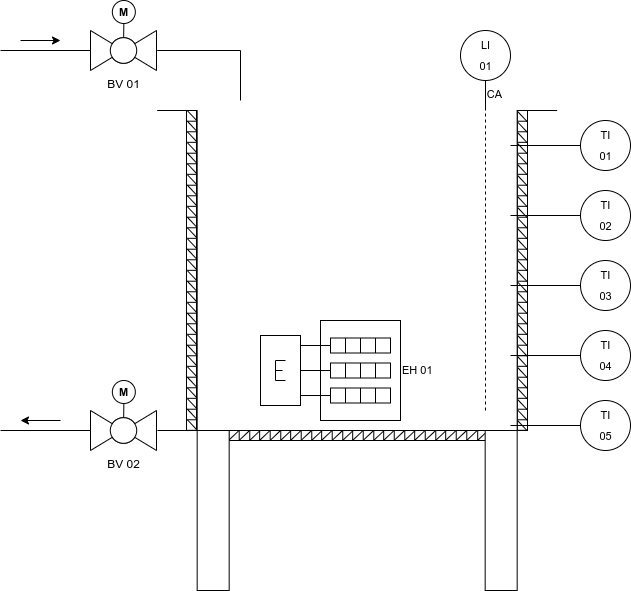
\includegraphics[width=0.8\textwidth]{imagens/tank.png}
    \caption{Diagrama dos transdutores e atuadores projetados para o tanque.}
    \label{fig:imagens-tank-png}
\end{figure}

Como pode-se ver, 5 transdutores de temperatura (TI 01 a 05) foram projetados para que seja possível o acompanhamento da temperatura ao longo do corpo do líquido, de forma a entender a distribuição de calor no mesmo. Além disso, um aquecedor (EH 01) interno foi projetado para que seja possível controlar a temperatura de saída do líquido. Para a vazão, duas válvulas (BV 01 e 02) e um transdutor de nível (LI 01) são esperados.

